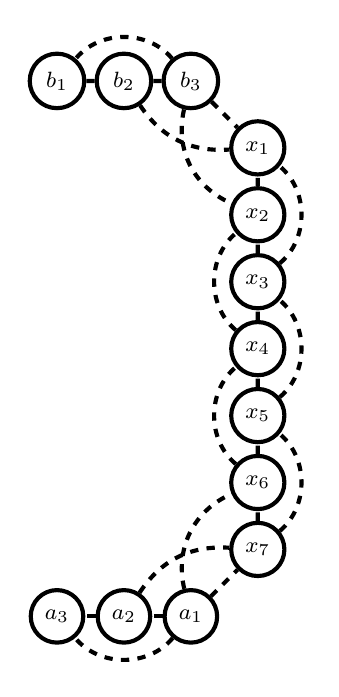
\begin{tikzpicture}[scale=0.85]
    \node[circle, draw=black, fill=white, line width=1.5pt, font=\footnotesize] (a2) at (0, 0) {$a_{3}$};
    \node[circle, draw=black, fill=white, line width=1.5pt, font=\footnotesize] (a1) at (1, 0) {$a_{2}$};
    \node[circle, draw=black, fill=white, line width=1.5pt, font=\footnotesize] (a0) at (2, 0) {$a_{1}$};

    \node[circle, draw=black, fill=white, line width=1.5pt, font=\footnotesize] (b2) at (0, 8) {$b_1$};
    \node[circle, draw=black, fill=white, line width=1.5pt, font=\footnotesize] (b1) at (1, 8) {$b_2$};
    \node[circle, draw=black, fill=white, line width=1.5pt, font=\footnotesize] (b0) at (2, 8) {$b_3$};
    
    \node[circle, draw=black, fill=white, line width=1.5pt, font=\footnotesize] (x1) at (3, 1) {$x_{7}$};
    \node[circle, draw=black, fill=white, line width=1.5pt, font=\footnotesize] (x2) at (3, 2) {$x_{6}$};
    \node[circle, draw=black, fill=white, line width=1.5pt, font=\footnotesize] (x3) at (3, 3) {$x_{5}$};
    \node[circle, draw=black, fill=white, line width=1.5pt, font=\footnotesize] (x4) at (3, 4) {$x_{4}$};
    \node[circle, draw=black, fill=white, line width=1.5pt, font=\footnotesize] (x5) at (3, 5) {$x_{3}$};
    \node[circle, draw=black, fill=white, line width=1.5pt, font=\footnotesize] (x6) at (3, 6) {$x_{2}$};
    \node[circle, draw=black, fill=white, line width=1.5pt, font=\footnotesize] (x7) at (3, 7) {$x_{1}$};
    
    \draw[line width=1.5pt, dashed] (a0) to (a1);
    \draw[line width=1.5pt, dashed] (a1) to (a2);
    \draw[line width=1.5pt, bend left=50, dashed] (a0) to (a2);

    \draw[line width=1.5pt, dashed] (b0) to (b1);
    \draw[line width=1.5pt, dashed] (b1) to (b2);
    \draw[line width=1.5pt, bend right=50, dashed] (b0) to (b2);


    \draw[line width=1.5pt, dashed] (x1) to (x2);
    \draw[line width=1.5pt, dashed] (x2) to (x3);
    \draw[line width=1.5pt, dashed] (x3) to (x4);
    \draw[line width=1.5pt, dashed] (x4) to (x5);
    \draw[line width=1.5pt, dashed] (x5) to (x6);
    \draw[line width=1.5pt, dashed] (x6) to (x7);

    \draw[line width=1.5pt, bend right=50, dashed] (x1) to (x3);
    \draw[line width=1.5pt, bend left=50, dashed] (x2) to (x4);
    \draw[line width=1.5pt, bend right=50, dashed] (x3) to (x5);
    \draw[line width=1.5pt, bend left=50, dashed] (x4) to (x6);
    \draw[line width=1.5pt, bend right=50, dashed] (x5) to (x7);

    \draw[line width=1.5pt, dashed] (a0) to (x1);
    \draw[line width=1.5pt, bend left=40, dashed] (a0) to (x2);
    \draw[line width=1.5pt, dashed, bend left=30,] (a1) to (x1);

    \draw[line width=1.5pt, dashed] (b0) to (x7);
    \draw[line width=1.5pt, bend right=40, dashed] (b0) to (x6);
    \draw[line width=1.5pt, dashed, bend right=30] (b1) to (x7);
\end{tikzpicture}